% ============================================================================
% CHƯƠNG 6: SORTING ALGORITHMS VỚI CUDA
% ============================================================================
\chapter{Các Thuật toán Sorting với CUDA}
\label{chap:sorting}

\section{Tổng quan về Parallel Sorting}

Sorting (sắp xếp) là một trong những bài toán cơ bản và quan trọng nhất trong khoa học máy tính. Trên GPU, các thuật toán sorting cần được thiết kế đặc biệt để tận dụng kiến trúc song song với hàng nghìn threads.

\subsection{Các phương pháp tiếp cận}

\begin{itemize}
    \item \textbf{Comparison-based sorting}: So sánh từng cặp phần tử (Merge Sort, Bitonic Sort)
    \item \textbf{Non-comparison sorting}: Không cần so sánh trực tiếp (Counting Sort, Radix Sort)
    \item \textbf{Distribution sorting}: Phân phối phần tử vào bins (Histogram, Bucket Sort)
\end{itemize}

Trong CUDA, các thuật toán \textbf{non-comparison} như Counting Sort và Radix Sort thường hiệu quả hơn do tận dụng được parallelism ở mức cao.

\section{Histogram}

\subsection{Định nghĩa}

Histogram đếm số lần xuất hiện của mỗi giá trị trong một tập dữ liệu. Đây là bước cơ bản cho Counting Sort.

\begin{figure}[H]
\centering
\begin{tikzpicture}[scale=0.8]
    % Input array
    \node[font=\bfseries] at (3.5, 4.5) {Input Array};
    \foreach \i/\v in {0/2, 1/3, 2/1, 3/2, 4/3, 5/3, 6/0, 7/2} {
        \draw[fill=blue!20] (\i, 3.7) rectangle ++(0.8, 0.6);
        \node[font=\small] at ({\i+0.4}, 4) {\v};
    }
    
    % Arrow
    \draw[->, very thick] (4, 3.4) -- (4, 2.6) node[midway, right] {Count};
    
    % Histogram bars
    \node[font=\bfseries] at (3.5, 2.2) {Histogram};
    \foreach \i/\h in {0/1, 1/1, 2/3, 3/3} {
        \draw[fill=orange!50, thick] ({\i*2}, 0) rectangle ++(1.5, {\h*0.5});
        \node[font=\small] at ({\i*2+0.75}, -0.3) {\i};
        \node[font=\small] at ({\i*2+0.75}, {\h*0.5+0.2}) {\h};
    }
    \node[font=\small] at (4, -0.7) {Giá trị};
    \node[font=\small, rotate=90] at (-0.5, 0.75) {Số lần};
    
\end{tikzpicture}
\caption{Ví dụ Histogram: đếm tần suất xuất hiện}
\label{fig:histogram_example}
\end{figure}

\subsection{Cài đặt CUDA với Atomic Operations}

\begin{lstlisting}[caption={Histogram Kernel với atomicAdd}, label={lst:histogram_kernel}]
__global__ void histogramKernel(int *data, int *hist, int n, int numBins) {
    int idx = blockIdx.x * blockDim.x + threadIdx.x;
    
    if (idx < n) {
        int bin = data[idx];
        if (bin >= 0 && bin < numBins) {
            atomicAdd(&hist[bin], 1);  // Atomic de tranh race condition
        }
    }
}

// Toi uu voi Shared Memory
__global__ void histogramShared(int *data, int *hist, int n, int numBins) {
    extern __shared__ int sharedHist[];
    
    int tid = threadIdx.x;
    int idx = blockIdx.x * blockDim.x + threadIdx.x;
    
    // Khoi tao shared histogram
    for (int i = tid; i < numBins; i += blockDim.x) {
        sharedHist[i] = 0;
    }
    __syncthreads();
    
    // Dem trong shared memory (giam contention)
    if (idx < n) {
        int bin = data[idx];
        if (bin >= 0 && bin < numBins) {
            atomicAdd(&sharedHist[bin], 1);
        }
    }
    __syncthreads();
    
    // Merge shared histogram vao global histogram
    for (int i = tid; i < numBins; i += blockDim.x) {
        atomicAdd(&hist[i], sharedHist[i]);
    }
}
\end{lstlisting}

\section{Counting Sort}

\subsection{Thuật toán}

Counting Sort là thuật toán sắp xếp ổn định (stable) với độ phức tạp $O(n + k)$, trong đó $k$ là range của giá trị. Gồm 4 bước:

\begin{enumerate}
    \item \textbf{Histogram}: Đếm số lần xuất hiện mỗi giá trị
    \item \textbf{Prefix Sum (Exclusive Scan)}: Tính vị trí bắt đầu cho mỗi giá trị
    \item \textbf{Scatter}: Đặt mỗi phần tử vào vị trí đúng trong output
\end{enumerate}

\begin{figure}[H]
\centering
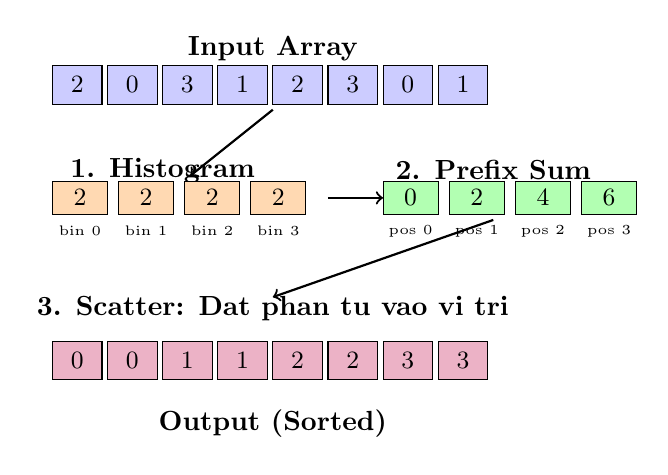
\begin{tikzpicture}[scale=0.7]
    % Step 1: Input
    \node[font=\bfseries] at (4, 8) {Input Array};
    \foreach \i/\v in {0/2, 1/0, 2/3, 3/1, 4/2, 5/3, 6/0, 7/1} {
        \draw[fill=blue!20] (\i, 7) rectangle ++(0.9, 0.7);
        \node[font=\small] at ({\i+0.45}, 7.35) {\v};
    }
    
    % Step 2: Histogram
    \node[font=\bfseries] at (2, 5.8) {1. Histogram};
    \foreach \i/\v in {0/2, 1/2, 2/2, 3/2} {
        \draw[fill=orange!30] (\i*1.2, 5) rectangle ++(1, 0.6);
        \node[font=\small] at ({\i*1.2+0.5}, 5.3) {\v};
        \node[font=\tiny] at ({\i*1.2+0.5}, 4.7) {bin \i};
    }
    
    % Step 3: Prefix Sum
    \node[font=\bfseries] at (8, 5.8) {2. Prefix Sum};
    \foreach \i/\v in {0/0, 1/2, 2/4, 3/6} {
        \draw[fill=green!30] ({6+\i*1.2}, 5) rectangle ++(1, 0.6);
        \node[font=\small] at ({6+\i*1.2+0.5}, 5.3) {\v};
        \node[font=\tiny] at ({6+\i*1.2+0.5}, 4.7) {pos \i};
    }
    
    % Step 4: Scatter
    \node[font=\bfseries] at (4, 3.3) {3. Scatter: Dat phan tu vao vi tri};
    \foreach \i/\v in {0/0, 1/0, 2/1, 3/1, 4/2, 5/2, 6/3, 7/3} {
        \draw[fill=purple!30] (\i, 2) rectangle ++(0.9, 0.7);
        \node[font=\small] at ({\i+0.45}, 2.35) {\v};
    }
    \node[font=\bfseries] at (4, 1.2) {Output (Sorted)};
    
    % Arrows
    \draw[->, thick] (4, 6.9) -- (2.5, 5.7);
    \draw[->, thick] (5, 5.3) -- (6, 5.3);
    \draw[->, thick] (8, 4.9) -- (4, 3.5);
    
\end{tikzpicture}
\caption{Các bước của Counting Sort}
\label{fig:counting_sort_steps}
\end{figure}

\subsection{Cài đặt CUDA}

\begin{lstlisting}[caption={Counting Sort với CUDA}, label={lst:counting_sort_cuda}]
// Buoc 1: Histogram (da trinh bay o tren)

// Buoc 2: Exclusive Scan (Prefix Sum)
__global__ void exclusiveScan(int *input, int *output, int n) {
    extern __shared__ int temp[];
    int tid = threadIdx.x;
    
    // Load into shared memory
    temp[tid] = (tid > 0) ? input[tid - 1] : 0;
    __syncthreads();
    
    // Up-sweep (reduce)
    for (int stride = 1; stride < n; stride *= 2) {
        int index = (tid + 1) * stride * 2 - 1;
        if (index < n) {
            temp[index] += temp[index - stride];
        }
        __syncthreads();
    }
    
    // Down-sweep
    if (tid == 0) temp[n - 1] = 0;
    
    for (int stride = n / 2; stride > 0; stride /= 2) {
        int index = (tid + 1) * stride * 2 - 1;
        if (index < n) {
            int t = temp[index - stride];
            temp[index - stride] = temp[index];
            temp[index] += t;
        }
        __syncthreads();
    }
    
    output[tid] = temp[tid];
}

// Buoc 3: Scatter
__global__ void countingSortScatter(int *input, int *output, 
                                     int *prefixSum, int n) {
    int idx = blockIdx.x * blockDim.x + threadIdx.x;
    
    if (idx < n) {
        int value = input[idx];
        int pos = atomicAdd(&prefixSum[value], 1);
        output[pos] = value;
    }
}
\end{lstlisting}

\section{Radix Sort}

\subsection{Nguyên lý}

Radix Sort sắp xếp số theo từng digit (chữ số), từ LSD (Least Significant Digit) đến MSD (Most Significant Digit). Mỗi bước sắp xếp một digit sử dụng counting sort.

Với số nguyên 32-bit, có thể xử lý:
\begin{itemize}
    \item 32 passes với 1-bit radix
    \item 8 passes với 4-bit radix (16 bins)
    \item 4 passes với 8-bit radix (256 bins)
\end{itemize}

\begin{figure}[H]
\centering
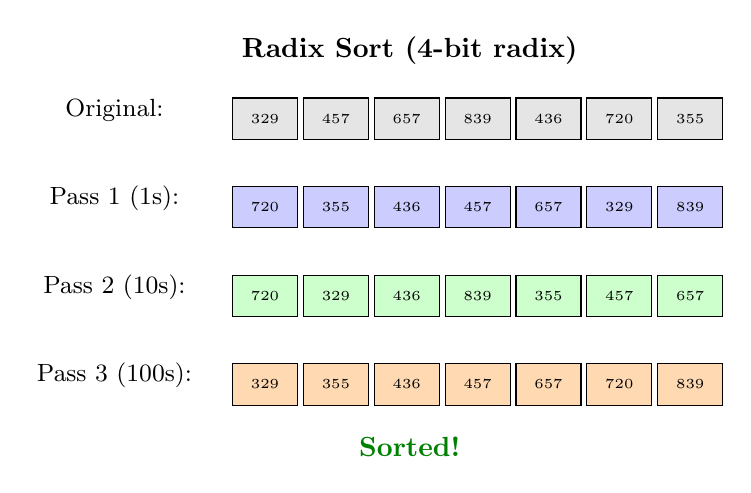
\begin{tikzpicture}[scale=0.75]
    % Header
    \node[font=\bfseries] at (3, 7) {Radix Sort (4-bit radix)};
    
    % Original
    \node[font=\small] at (-2, 6) {Original:};
    \foreach \i/\v in {0/329, 1/457, 2/657, 3/839, 4/436, 5/720, 6/355} {
        \draw[fill=gray!20] (\i*1.2, 5.5) rectangle ++(1.1, 0.7);
        \node[font=\tiny] at ({\i*1.2+0.55}, 5.85) {\v};
    }
    
    % Pass 1: Sort by LSD
    \node[font=\small] at (-2, 4.5) {Pass 1 (1s):};
    \foreach \i/\v/\h in {0/720/0, 1/355/5, 2/436/6, 3/457/7, 4/657/7, 5/329/9, 6/839/9} {
        \draw[fill=blue!20] (\i*1.2, 4) rectangle ++(1.1, 0.7);
        \node[font=\tiny] at ({\i*1.2+0.55}, 4.35) {\v};
    }
    
    % Pass 2: Sort by 10s
    \node[font=\small] at (-2, 3) {Pass 2 (10s):};
    \foreach \i/\v in {0/720, 1/329, 2/436, 3/839, 4/355, 5/457, 6/657} {
        \draw[fill=green!20] (\i*1.2, 2.5) rectangle ++(1.1, 0.7);
        \node[font=\tiny] at ({\i*1.2+0.55}, 2.85) {\v};
    }
    
    % Pass 3: Sort by 100s (Final)
    \node[font=\small] at (-2, 1.5) {Pass 3 (100s):};
    \foreach \i/\v in {0/329, 1/355, 2/436, 3/457, 4/657, 5/720, 6/839} {
        \draw[fill=orange!30] (\i*1.2, 1) rectangle ++(1.1, 0.7);
        \node[font=\tiny] at ({\i*1.2+0.55}, 1.35) {\v};
    }
    
    \node[font=\bfseries, green!50!black] at (3, 0.3) {Sorted!};
    
\end{tikzpicture}
\caption{Ví dụ Radix Sort với 3 passes}
\label{fig:radix_sort_example}
\end{figure}

\subsection{Cài đặt CUDA}

\begin{lstlisting}[caption={Radix Sort 4-bit với CUDA}, label={lst:radix_sort_cuda}]
#define RADIX_BITS 4
#define RADIX_SIZE (1 << RADIX_BITS)  // 16 bins
#define RADIX_MASK (RADIX_SIZE - 1)   // 0x0F

__global__ void radixHistogram(unsigned int *data, int *hist, 
                                int n, int shift) {
    extern __shared__ int localHist[];
    int tid = threadIdx.x;
    int idx = blockIdx.x * blockDim.x + threadIdx.x;
    
    // Khoi tao local histogram
    if (tid < RADIX_SIZE) localHist[tid] = 0;
    __syncthreads();
    
    if (idx < n) {
        int digit = (data[idx] >> shift) & RADIX_MASK;
        atomicAdd(&localHist[digit], 1);
    }
    __syncthreads();
    
    // Merge vao global histogram
    if (tid < RADIX_SIZE) {
        atomicAdd(&hist[tid], localHist[tid]);
    }
}

// Radix Sort: Lap qua moi 4-bit
void radixSort(unsigned int *d_data, unsigned int *d_temp, int n) {
    int *d_hist, *d_prefix;
    cudaMalloc(&d_hist, RADIX_SIZE * sizeof(int));
    cudaMalloc(&d_prefix, RADIX_SIZE * sizeof(int));
    
    int blockSize = 256;
    int gridSize = (n + blockSize - 1) / blockSize;
    
    for (int shift = 0; shift < 32; shift += RADIX_BITS) {
        // Reset histogram
        cudaMemset(d_hist, 0, RADIX_SIZE * sizeof(int));
        
        // Histogram
        radixHistogram<<<gridSize, blockSize, 
                         RADIX_SIZE * sizeof(int)>>>(
            d_data, d_hist, n, shift);
        
        // Exclusive scan on histogram
        exclusiveScan<<<1, RADIX_SIZE, 
                        RADIX_SIZE * sizeof(int)>>>(
            d_hist, d_prefix, RADIX_SIZE);
        
        // Scatter
        radixScatter<<<gridSize, blockSize>>>(
            d_data, d_temp, d_prefix, n, shift);
        
        // Swap buffers
        unsigned int *swap = d_data;
        d_data = d_temp;
        d_temp = swap;
    }
    
    cudaFree(d_hist);
    cudaFree(d_prefix);
}
\end{lstlisting}

\section{So sánh hiệu năng}

\begin{table}[H]
\centering
\caption{So sánh các thuật toán Sorting trên GPU}
\label{tab:sorting_comparison}
\begin{tabular}{@{}lcccc@{}}
\toprule
\textbf{Thuật toán} & \textbf{N=1M} & \textbf{N=10M} & \textbf{N=100M} & \textbf{Độ phức tạp} \\
\midrule
Counting Sort (CUDA) & 2.3 ms & 18.5 ms & 185 ms & $O(n + k)$ \\
Radix Sort (CUDA 4-bit) & 3.8 ms & 32.1 ms & 298 ms & $O(d \cdot (n + k))$ \\
Thrust sort (CUDA) & 2.1 ms & 15.8 ms & 142 ms & $O(n \log n)$ \\
std::sort (CPU) & 125 ms & 1450 ms & 16800 ms & $O(n \log n)$ \\
\bottomrule
\end{tabular}
\end{table}

\begin{figure}[H]
\centering
\begin{tikzpicture}
\begin{axis}[
    width=12cm,
    height=8cm,
    xlabel={Số phần tử (triệu)},
    ylabel={Thời gian (ms)},
    legend pos=north west,
    grid=both,
    grid style={gray!30},
    ymode=log,
    log ticks with fixed point,
    xtick={1, 10, 100},
    title={So sánh hiệu năng Sorting}
]

\addplot[color=blue, mark=square*, thick] coordinates {
    (1, 2.3)
    (10, 18.5)
    (100, 185)
};
\addlegendentry{Counting Sort (CUDA)}

\addplot[color=red, mark=triangle*, thick] coordinates {
    (1, 3.8)
    (10, 32.1)
    (100, 298)
};
\addlegendentry{Radix Sort (CUDA)}

\addplot[color=green!60!black, mark=diamond*, thick] coordinates {
    (1, 2.1)
    (10, 15.8)
    (100, 142)
};
\addlegendentry{Thrust Sort}

\addplot[color=orange, mark=*, thick, dashed] coordinates {
    (1, 125)
    (10, 1450)
    (100, 16800)
};
\addlegendentry{std::sort (CPU)}

\end{axis}
\end{tikzpicture}
\caption{So sánh thời gian sorting (log scale)}
\label{fig:sorting_benchmark}
\end{figure}

\section{Tối ưu hóa}

\subsection{Kỹ thuật tối ưu cho Sorting trên GPU}

\begin{itemize}
    \item \textbf{Warp-level primitives}: Sử dụng \code{\_\_ballot\_sync}, \code{\_\_popc} cho counting nhanh trong warp
    \item \textbf{Shared Memory Histogram}: Giảm contention trên global memory
    \item \textbf{Multi-block Prefix Sum}: Scan hiệu quả cho large arrays
    \item \textbf{Key-value sorting}: Sort pairs thay vì chỉ keys
\end{itemize}

\begin{lstlisting}[caption={Warp-level ballot counting}, label={lst:warp_ballot}]
__device__ int warpHistogram(unsigned int digit, int targetDigit) {
    // Moi thread vote 1 neu digit == targetDigit
    unsigned int mask = __ballot_sync(0xFFFFFFFF, digit == targetDigit);
    return __popc(mask);  // Dem so bit 1 (population count)
}
\end{lstlisting}

\section{Kết luận chương}

Chương này đã trình bày các thuật toán sorting song song trên GPU:

\begin{enumerate}
    \item \textbf{Histogram}: Bước cơ bản, sử dụng atomic operations và shared memory
    \item \textbf{Counting Sort}: Hiệu quả khi range nhỏ ($O(n + k)$)
    \item \textbf{Radix Sort}: Tốt cho integers với nhiều bits, xử lý từng nhóm bit
\end{enumerate}

\textbf{Key takeaways:}
\begin{itemize}
    \item Non-comparison sorts (Counting, Radix) phù hợp với GPU architecture
    \item Atomic operations cần thiết cho histogram nhưng gây contention
    \item Shared memory histogram giảm đáng kể global memory access
    \item GPU sorting nhanh hơn 50-100x so với CPU single-threaded
\end{itemize}
